\section{Numerical verification of the local theory}

The theoretical predictions were tested on a grounded \(5\times5\) square-grid
network with \(24\) free nodes and \(M=40\) adaptive edges. One corner node was
grounded, the conductances were sampled independently from
\([0.75,1.25]\), and the random seed was fixed at \(260613\). All reported
quantities and figures are generated by the accompanying reproducible Python
implementation.

\subsection{Verification of the sensitivity identity}

The analytical graph-Laplacian Jacobian was compared with PyTorch automatic
differentiation and centred finite differences. The relative discrepancy
between the analytical and automatically differentiated Jacobians was
\[
    6.51\times10^{-15},
\]
which is at the level of double-precision round-off. The best centred
finite-difference approximation occurred at
\[
    \varepsilon=2.15\times10^{-5},
\]
with relative error
\[
    5.60\times10^{-10}.
\]
These results verify the identity
\[
    \frac{\partial y_A}{\partial g_e}
    =
    -C_AL(g)^{-1}b_e\,b_e^Tu_A
\]
to numerical precision.

\begin{figure}[H]
\centering
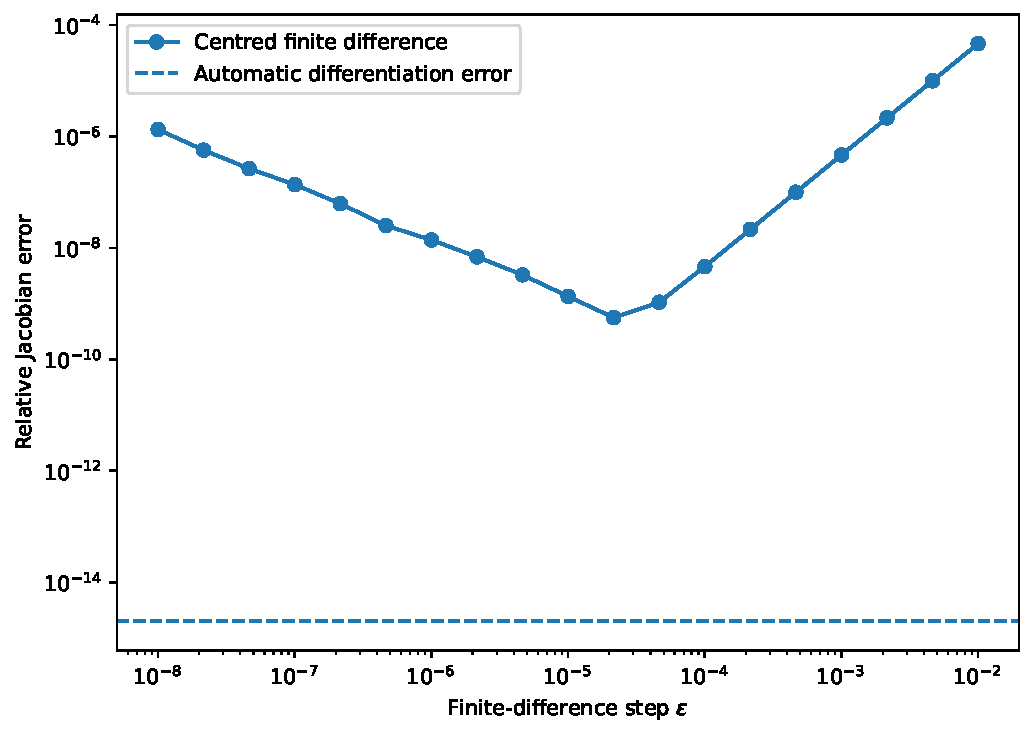
\includegraphics[width=0.76\textwidth]
{results/theory_verification/figures/figure_sensitivity_identity.pdf}
\caption{Relative error in the graph-Laplacian sensitivity identity. The
analytical Jacobian agrees with automatic differentiation to machine precision,
while centred finite differences display the expected truncation--round-off
trade-off.}
\label{fig:sensitivity_identity}
\end{figure}

\subsection{Quadratic and quartic forgetting laws}

For sensitive-subspace perturbations \(\Delta g=\varepsilon v_\parallel\),
the measured forgetting had fitted log--log slope
\[
    2.006,
\]
in agreement with the quadratic law
\[
    F_A(\varepsilon v_\parallel)
    =
    \frac{\varepsilon^2}{2}
    \|J_Av_\parallel\|^2
    +O(\varepsilon^3).
\]
The absolute error between the nonlinear forgetting and the quadratic
prediction had fitted slope
\[
    3.006,
\]
confirming the cubic Taylor remainder.

\begin{figure}[H]
\centering
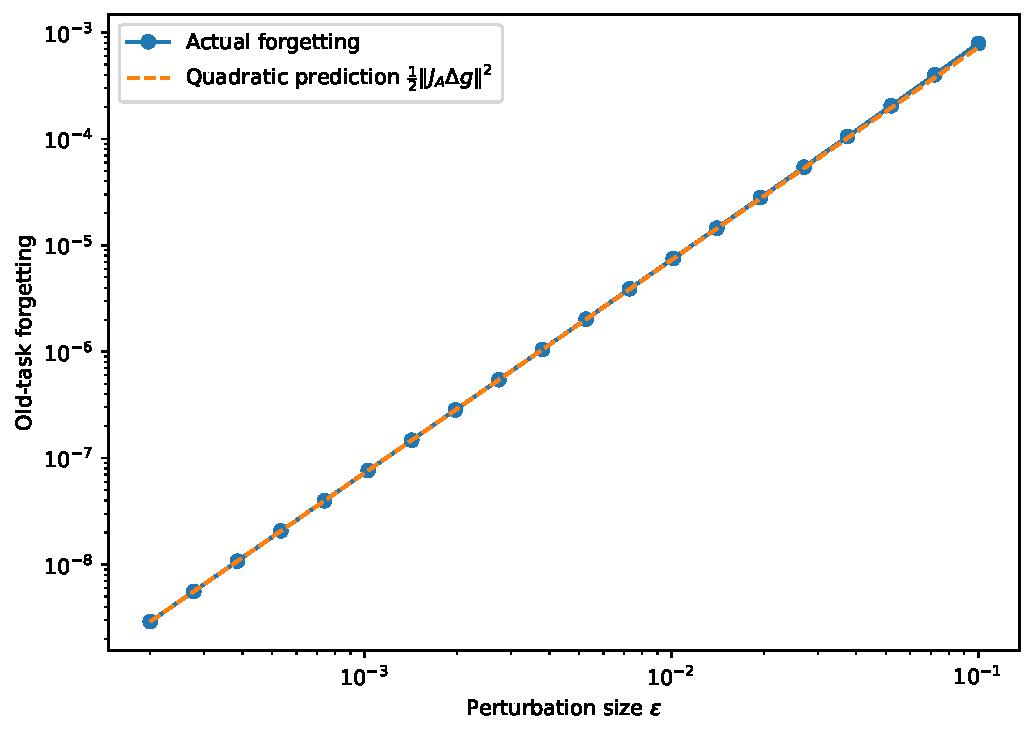
\includegraphics[width=0.76\textwidth]
{results/theory_verification/figures/figure_quadratic_forgetting.pdf}
\caption{Actual old-task forgetting and the quadratic prediction
\(\frac12\|J_A\Delta g\|^2\). The two curves agree throughout the local
perturbation regime.}
\label{fig:quadratic_forgetting}
\end{figure}

\begin{figure}[H]
\centering
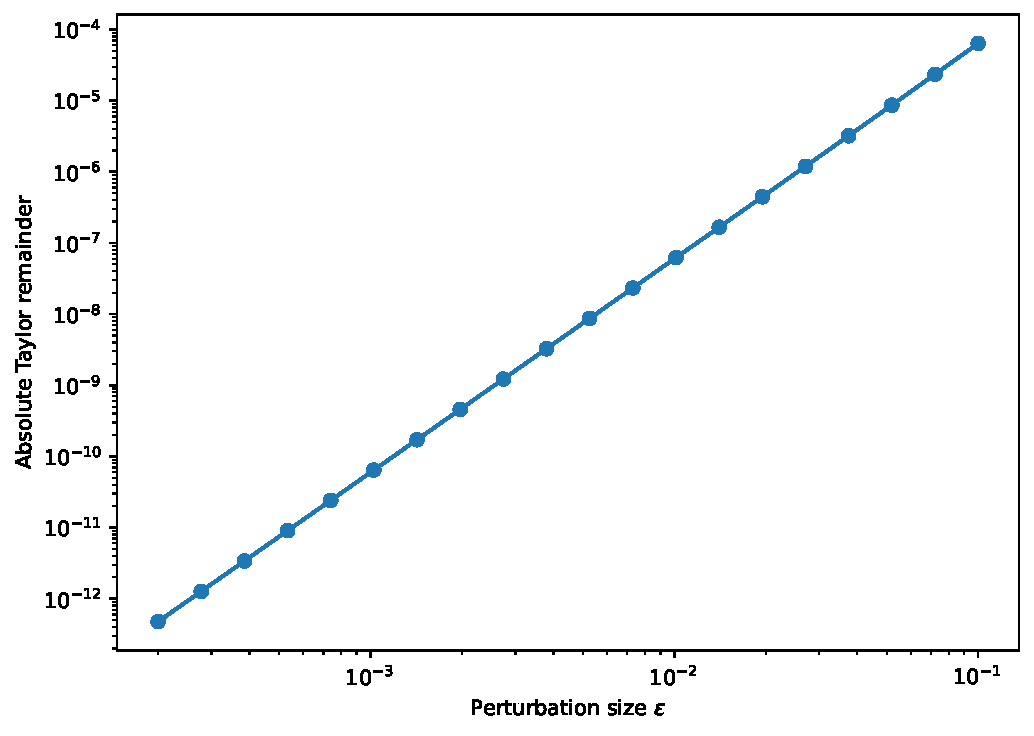
\includegraphics[width=0.76\textwidth]
{results/theory_verification/figures/figure_quadratic_remainder.pdf}
\caption{Absolute remainder in the quadratic forgetting approximation. The
fitted log--log slope is \(3.006\), consistent with an
\(O(\|\Delta g\|^3)\) remainder.}
\label{fig:quadratic_remainder}
\end{figure}

For a numerically constructed null-space direction \(v_\perp\), the projection
residual was
\[
    \|J_Av_\perp\|=1.98\times10^{-17}.
\]
The corresponding forgetting had fitted slope
\[
    4.002,
\]
which verifies the sharper null-space law
\[
    F_A(\varepsilon v_\perp)=O(\varepsilon^4).
\]
Thus, equal-norm perturbations in the sensitive and null subspaces produce
quadratically and quartically small forgetting, respectively.

\begin{figure}[H]
\centering
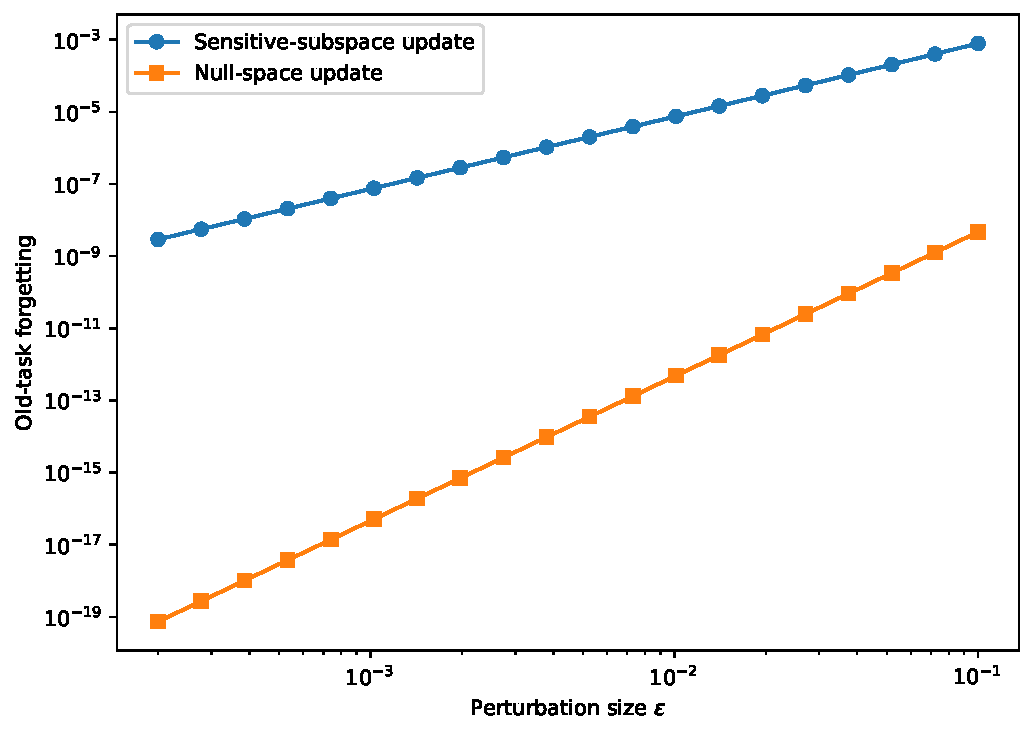
\includegraphics[width=0.76\textwidth]
{results/theory_verification/figures/figure_null_vs_sensitive.pdf}
\caption{Forgetting produced by equal-norm sensitive-subspace and null-space
perturbations. The fitted slopes are approximately \(2\) and \(4\),
respectively.}
\label{fig:null_vs_sensitive}
\end{figure}

\subsection{Rank exhaustion of first-order plasticity}

For independent randomly generated scalar tasks, the stacked sensitivity rank
increased by one per task until reaching the full conductance dimension
\[
    \operatorname{rank}\mathcal{J}_{40}=40.
\]
Accordingly, the first-order plastic dimension decreased from \(39\) after the
first task to zero after the fortieth independent task. In contrast, a sequence
constructed by repeatedly drawing from five sensitivity rows saturated at rank
\(5\), leaving a \(35\)-dimensional plastic subspace. This verifies that local
capacity is controlled by independent sensitivity rank rather than by the raw
number of tasks.

\begin{figure}[H]
\centering
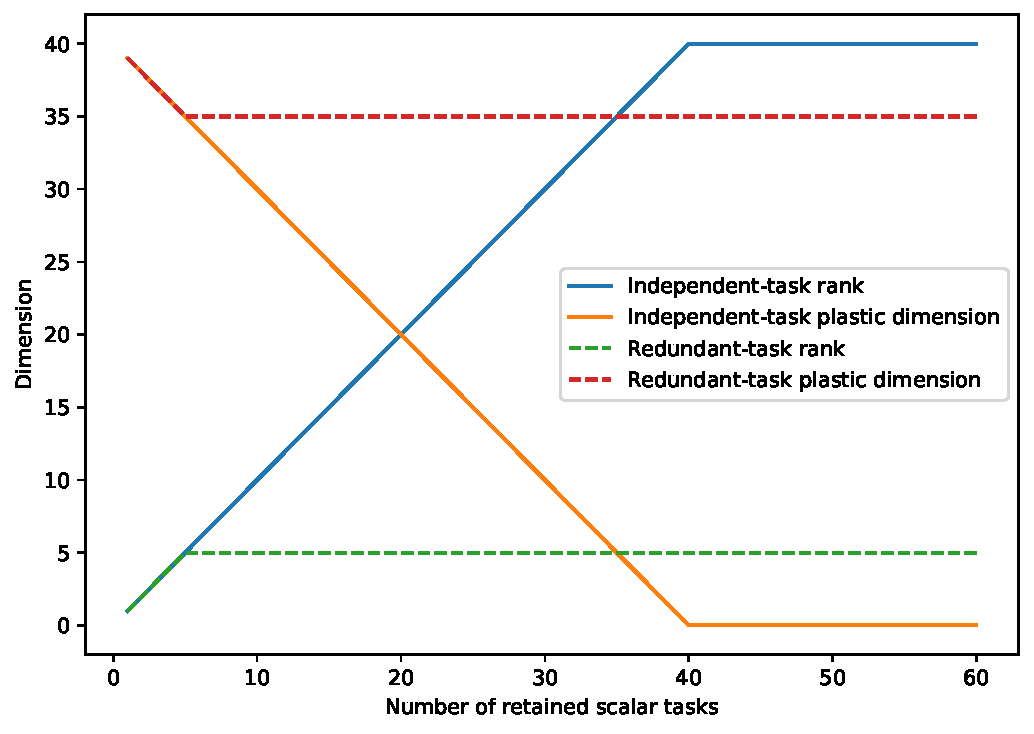
\includegraphics[width=0.76\textwidth]
{results/theory_verification/figures/figure_rank_capacity.pdf}
\caption{Growth of stacked sensitivity rank and loss of first-order plastic
dimension. Independent scalar tasks exhaust all \(40\) conductance directions,
whereas redundant tasks saturate at rank \(5\).}
\label{fig:rank_capacity}
\end{figure}

\subsection{Anchoring asymptotics and safe plasticity}

For uniform positive-definite anchoring, the fitted large-\(\lambda\) scaling of
the update norm was
\[
    \|\Delta g_\lambda\|\sim \lambda^{-0.9999},
\]
while old-task forgetting scaled as
\[
    F_A(\lambda)\sim \lambda^{-1.9979}.
\]
These values agree with the theoretical asymptotics
\[
    \|\Delta g_\lambda\|=O(\lambda^{-1}),
    \qquad
    F_A(\lambda)=O(\lambda^{-2}).
\]
At \(\lambda=10^5\), uniform anchoring reduced the update norm to
\(1.31\times10^{-8}\), but the new-task loss approached
\(2.50\times10^{-5}\), which is the unadapted loss. This confirms that strong
uniform anchoring protects memory by freezing adaptation.

Sensitivity anchoring behaved differently. At \(\lambda=10^5\), the update
norm remained \(1.94\times10^{-2}\), demonstrating persistent motion in the
old-task null space. The new-task loss was \(1.24\times10^{-5}\), approximately
half the uniform-anchor value, while the old-task forgetting was
\(1.02\times10^{-10}\). The quadratic forgetting prediction tends to zero in
this limit, whereas the nonlinear forgetting approaches a small quartic
plateau. This is the expected signature of safe first-order plasticity with
nonzero higher-order interference.

\begin{figure}[H]
\centering
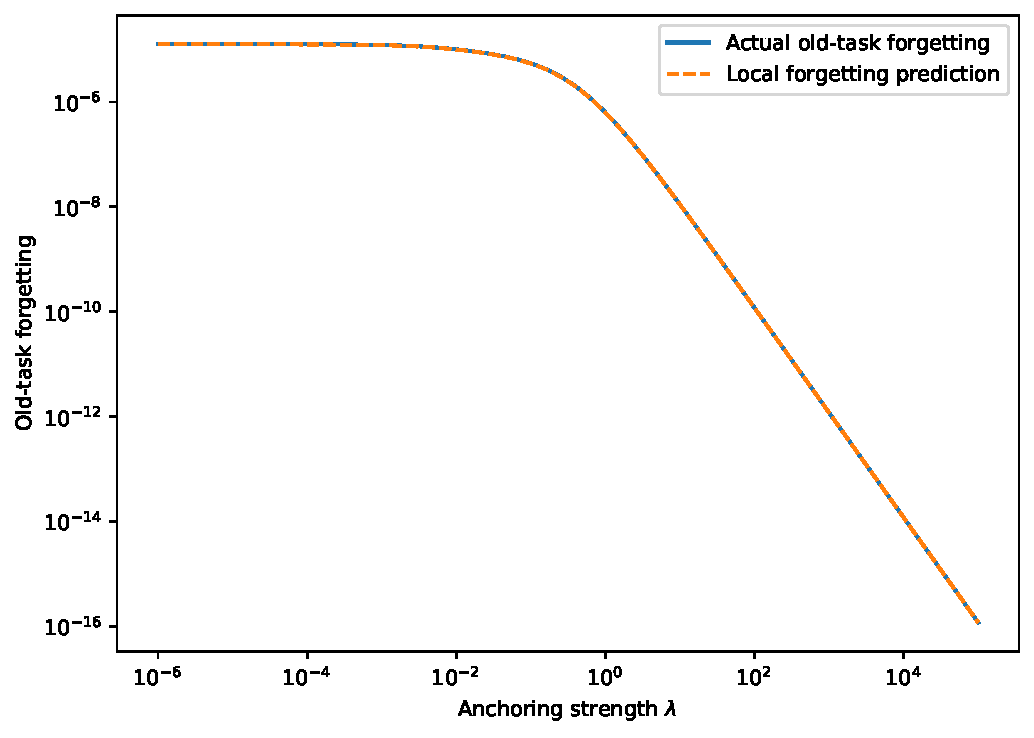
\includegraphics[width=0.76\textwidth]
{results/theory_verification/figures/figure_anchoring_formula_uniform.pdf}
\caption{Actual and predicted old-task forgetting under uniform anchoring. The
local prediction remains accurate and the large-\(\lambda\) decay is
quadratic.}
\label{fig:anchoring_uniform}
\end{figure}

\begin{figure}[H]
\centering
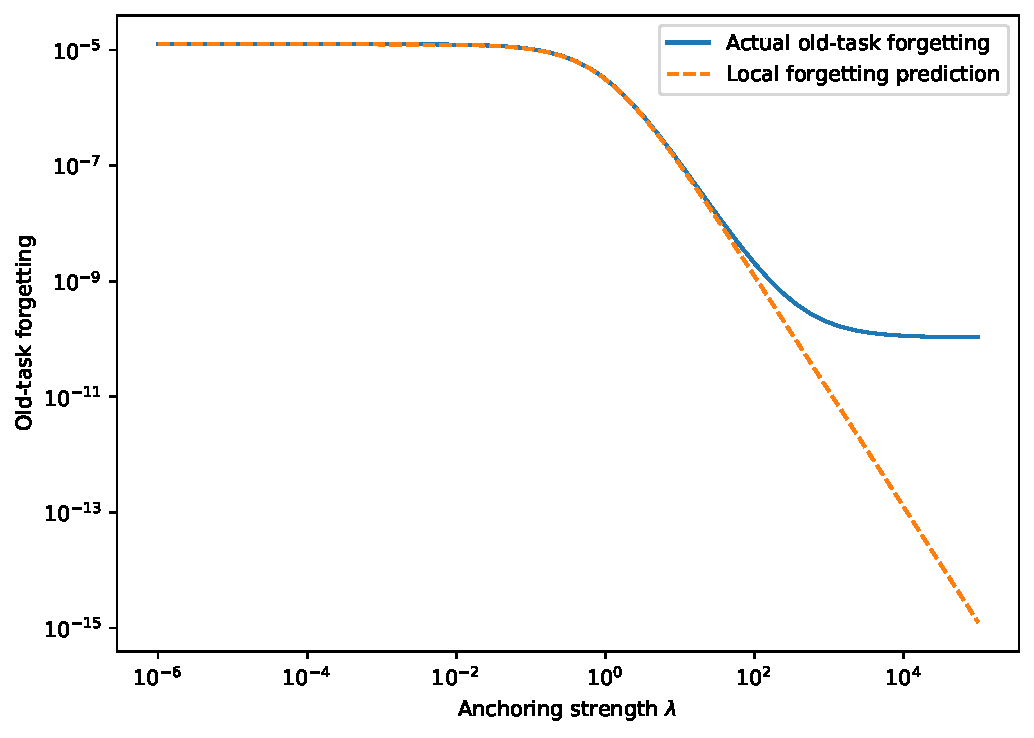
\includegraphics[width=0.76\textwidth]
{results/theory_verification/figures/figure_anchoring_formula_sensitivity.pdf}
\caption{Actual and predicted old-task forgetting under sensitivity anchoring.
The quadratic term is suppressed as \(\lambda\) increases, while the full
nonlinear forgetting approaches a small quartic plateau because the limiting
safe update remains nonzero.}
\label{fig:anchoring_sensitivity}
\end{figure}

\begin{figure}[H]
\centering
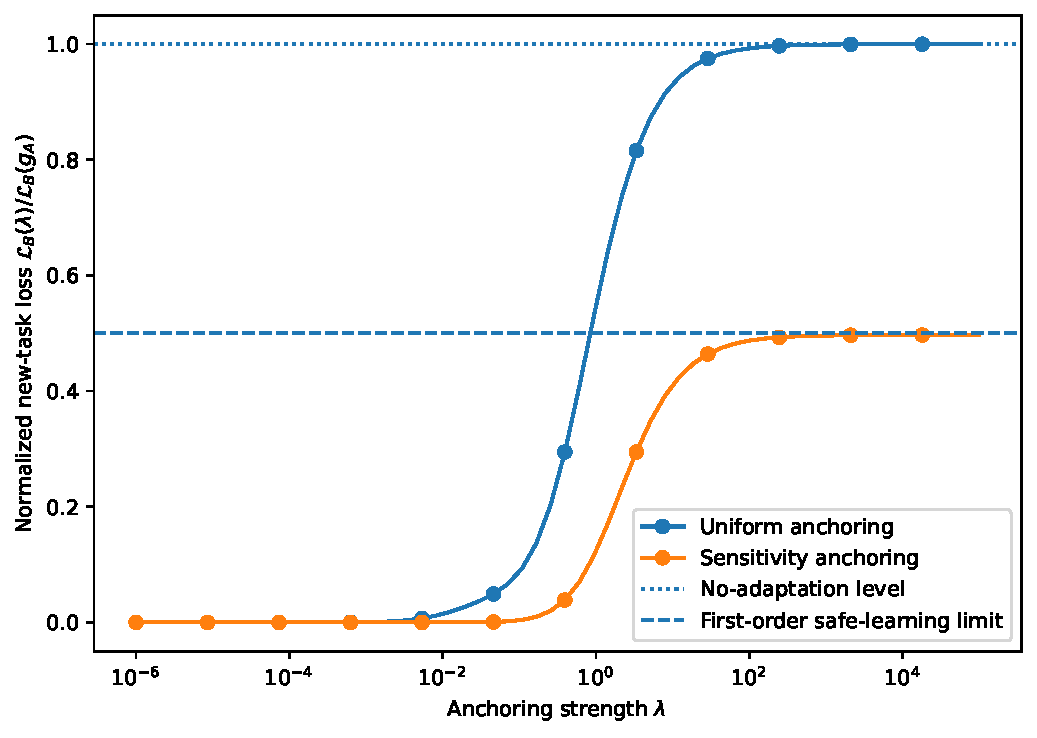
\includegraphics[width=0.76\textwidth]
{results/theory_verification/figures/figure_anchoring_tradeoff.pdf}
\caption{Adaptation--retention trade-off for uniform and sensitivity anchoring.
Sensitivity anchoring retains useful null-space adaptation at levels where
uniform anchoring has effectively frozen the network.}
\label{fig:anchoring_tradeoff}
\end{figure}

\subsection{Forward--adjoint pathway structure}

The correlation between edge-current magnitude and exact edge sensitivity was
\[
    0.617.
\]
The correlation is positive but far from unity. This confirms the theoretical
prediction that current alone is not a complete importance measure. Exact edge
sensitivity is the product of a forward voltage-drop factor and an adjoint
output-transfer factor,
\[
    s_{A,e}=|\theta_{A,e}\phi_{A,e}|.
\]

\begin{figure}[H]
\centering
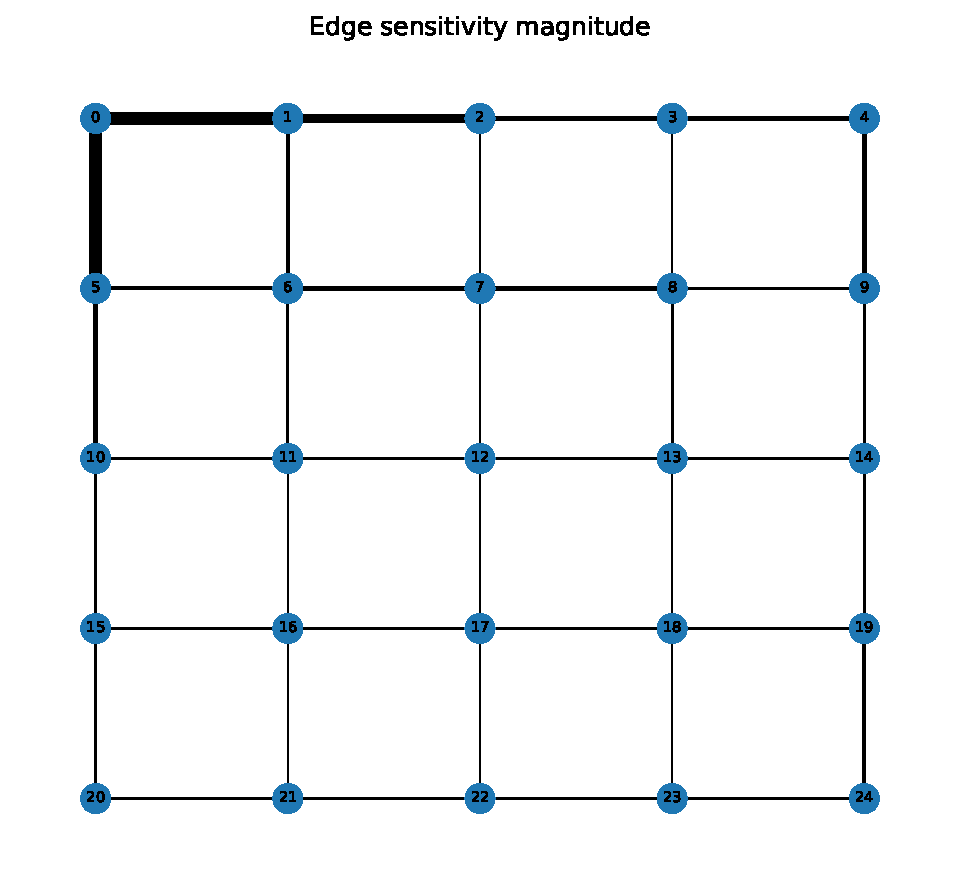
\includegraphics[width=0.76\textwidth]
{results/theory_verification/figures/figure_edge_sensitivity_map.pdf}
\caption{Edge sensitivity represented by line width. The sensitivity map is
controlled by overlap between the forward task response and the adjoint
response from the measured output.}
\label{fig:edge_sensitivity_map}
\end{figure}

The numerical results therefore verify all principal local predictions: the
exact conductance sensitivity identity, quadratic forgetting in sensitive
directions, quartic forgetting in null directions, rank-controlled exhaustion
of plasticity, and the distinct large-anchoring limits of uniform and
sensitivity-based consolidation.
